% Created by tikzDevice version 0.6.1 on 2016-02-05 02:08:14
% !TEX encoding = UTF-8 Unicode
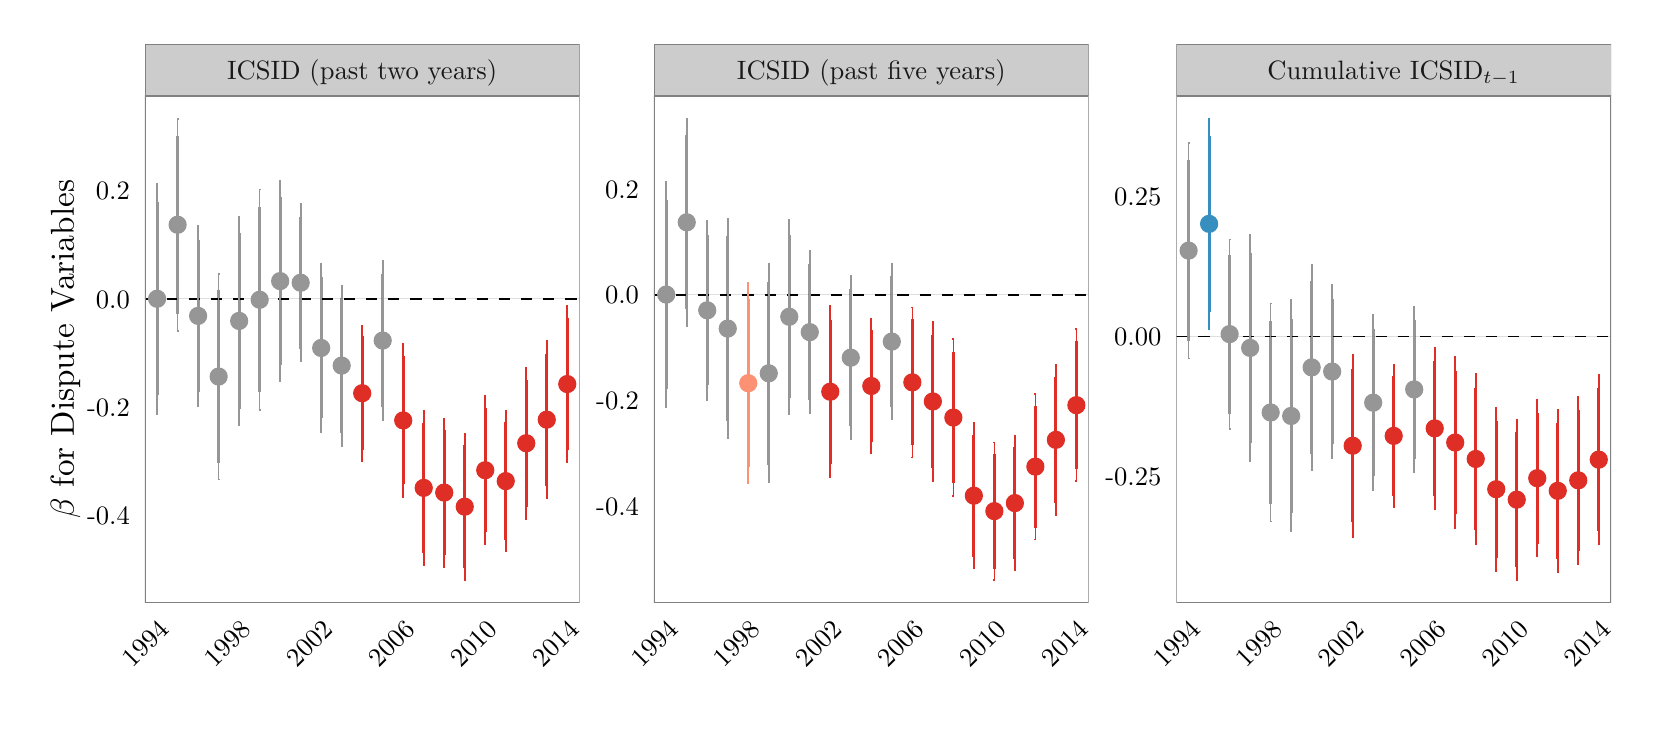
\begin{tikzpicture}[x=1pt,y=1pt]
\definecolor[named]{drawColor}{rgb}{0.00,0.00,0.00}
\definecolor[named]{fillColor}{rgb}{1.00,1.00,1.00}
\fill[color=fillColor,] (0,0) rectangle (578.16,252.94);
\begin{scope}
\path[clip] (  0.00,  0.00) rectangle (578.16,252.94);
\end{scope}
\begin{scope}
\path[clip] (  0.00,  0.00) rectangle (578.16,252.94);
\end{scope}
\begin{scope}
\path[clip] (  0.00,  0.00) rectangle (578.16,252.94);
\end{scope}
\begin{scope}
\path[clip] (  0.00,  0.00) rectangle (578.16,252.94);
\end{scope}
\begin{scope}
\path[clip] (  0.00,  0.00) rectangle (578.16,252.94);
\end{scope}
\begin{scope}
\path[clip] (  0.00,  0.00) rectangle (578.16,252.94);
\end{scope}
\begin{scope}
\path[clip] (  0.00,  0.00) rectangle (578.16,252.94);
\end{scope}
\begin{scope}
\path[clip] (  0.00,  0.00) rectangle (578.16,252.94);
\end{scope}
\begin{scope}
\path[clip] (  0.00,  0.00) rectangle (578.16,252.94);
\end{scope}
\begin{scope}
\path[clip] (  0.00,  0.00) rectangle (578.16,252.94);
\end{scope}
\begin{scope}
\path[clip] (  0.00,  0.00) rectangle (578.16,252.94);
\end{scope}
\begin{scope}
\path[clip] (  0.00,  0.00) rectangle (578.16,252.94);
\end{scope}
\begin{scope}
\path[clip] (  0.00,  0.00) rectangle (578.16,252.94);
\end{scope}
\begin{scope}
\path[clip] (  0.00,  0.00) rectangle (578.16,252.94);
\end{scope}
\begin{scope}
\path[clip] (  0.00,  0.00) rectangle (578.16,252.94);
\end{scope}
\begin{scope}
\path[clip] (  0.00,  0.00) rectangle (578.16,252.94);
\definecolor[named]{drawColor}{rgb}{1.00,1.00,1.00}
\definecolor[named]{fillColor}{rgb}{1.00,1.00,1.00}

\draw[color=drawColor,line width= 0.6pt,line cap=round,line join=round,fill=fillColor,] ( -0.00,  0.00) rectangle (578.16,252.94);
\end{scope}
\begin{scope}
\path[clip] (  0.00,  0.00) rectangle (578.16,252.94);
\end{scope}
\begin{scope}
\path[clip] ( 42.33, 45.11) rectangle (199.43,228.33);
\definecolor[named]{fillColor}{rgb}{1.00,1.00,1.00}

\draw[fill=fillColor,draw opacity=0.00,] ( 42.33, 45.11) rectangle (199.43,228.33);
\definecolor[named]{drawColor}{rgb}{0.59,0.59,0.59}
\definecolor[named]{fillColor}{rgb}{0.59,0.59,0.59}

\draw[color=drawColor,line width= 0.3pt,line join=round,fill=fillColor,fill opacity=0.30,draw opacity=0.30,] ( 46.77,113.41) -- ( 46.77,196.55);

\draw[color=drawColor,line width= 0.3pt,line join=round,fill=fillColor,fill opacity=0.30,draw opacity=0.30,] ( 54.18,143.43) -- ( 54.18,220.01);

\draw[color=drawColor,line width= 0.3pt,line join=round,fill=fillColor,fill opacity=0.30,draw opacity=0.30,] ( 61.59,116.08) -- ( 61.59,181.50);

\draw[color=drawColor,line width= 0.3pt,line join=round,fill=fillColor,fill opacity=0.30,draw opacity=0.30,] ( 69.01, 89.72) -- ( 69.01,164.02);

\draw[color=drawColor,line width= 0.3pt,line join=round,fill=fillColor,fill opacity=0.30,draw opacity=0.30,] ( 76.42,109.25) -- ( 76.42,184.69);

\draw[color=drawColor,line width= 0.3pt,line join=round,fill=fillColor,fill opacity=0.30,draw opacity=0.30,] ( 83.83,114.73) -- ( 83.83,194.50);

\draw[color=drawColor,line width= 0.3pt,line join=round,fill=fillColor,fill opacity=0.30,draw opacity=0.30,] ( 91.24,125.19) -- ( 91.24,197.53);

\draw[color=drawColor,line width= 0.3pt,line join=round,fill=fillColor,fill opacity=0.30,draw opacity=0.30,] ( 98.65,132.34) -- ( 98.65,189.19);

\draw[color=drawColor,line width= 0.3pt,line join=round,fill=fillColor,fill opacity=0.30,draw opacity=0.30,] (106.06,106.85) -- (106.06,167.55);

\draw[color=drawColor,line width= 0.3pt,line join=round,fill=fillColor,fill opacity=0.30,draw opacity=0.30,] (113.47,101.86) -- (113.47,159.82);
\definecolor[named]{drawColor}{rgb}{0.87,0.18,0.15}
\definecolor[named]{fillColor}{rgb}{0.87,0.18,0.15}

\draw[color=drawColor,line width= 0.3pt,line join=round,fill=fillColor,fill opacity=0.30,draw opacity=0.30,] (120.88, 96.35) -- (120.88,145.36);
\definecolor[named]{drawColor}{rgb}{0.59,0.59,0.59}
\definecolor[named]{fillColor}{rgb}{0.59,0.59,0.59}

\draw[color=drawColor,line width= 0.3pt,line join=round,fill=fillColor,fill opacity=0.30,draw opacity=0.30,] (128.29,111.20) -- (128.29,168.56);
\definecolor[named]{drawColor}{rgb}{0.87,0.18,0.15}
\definecolor[named]{fillColor}{rgb}{0.87,0.18,0.15}

\draw[color=drawColor,line width= 0.3pt,line join=round,fill=fillColor,fill opacity=0.30,draw opacity=0.30,] (135.70, 83.44) -- (135.70,138.59);

\draw[color=drawColor,line width= 0.3pt,line join=round,fill=fillColor,fill opacity=0.30,draw opacity=0.30,] (143.11, 58.80) -- (143.11,114.49);

\draw[color=drawColor,line width= 0.3pt,line join=round,fill=fillColor,fill opacity=0.30,draw opacity=0.30,] (150.52, 58.15) -- (150.52,111.73);

\draw[color=drawColor,line width= 0.3pt,line join=round,fill=fillColor,fill opacity=0.30,draw opacity=0.30,] (157.93, 53.44) -- (157.93,106.26);

\draw[color=drawColor,line width= 0.3pt,line join=round,fill=fillColor,fill opacity=0.30,draw opacity=0.30,] (165.34, 66.28) -- (165.34,119.76);

\draw[color=drawColor,line width= 0.3pt,line join=round,fill=fillColor,fill opacity=0.30,draw opacity=0.30,] (172.75, 63.62) -- (172.75,114.55);

\draw[color=drawColor,line width= 0.3pt,line join=round,fill=fillColor,fill opacity=0.30,draw opacity=0.30,] (180.16, 75.42) -- (180.16,130.11);

\draw[color=drawColor,line width= 0.3pt,line join=round,fill=fillColor,fill opacity=0.30,draw opacity=0.30,] (187.57, 82.92) -- (187.57,139.67);

\draw[color=drawColor,line width= 0.3pt,line join=round,fill=fillColor,fill opacity=0.30,draw opacity=0.30,] (194.98, 95.76) -- (194.98,152.55);
\definecolor[named]{drawColor}{rgb}{0.59,0.59,0.59}
\definecolor[named]{fillColor}{rgb}{0.59,0.59,0.59}

\draw[color=drawColor,line width= 1.1pt,line join=round,fill=fillColor,] ( 46.77,120.10) -- ( 46.77,189.86);

\draw[color=drawColor,line width= 1.1pt,line join=round,fill=fillColor,] ( 54.18,149.58) -- ( 54.18,213.85);

\draw[color=drawColor,line width= 1.1pt,line join=round,fill=fillColor,] ( 61.59,121.34) -- ( 61.59,176.25);

\draw[color=drawColor,line width= 1.1pt,line join=round,fill=fillColor,] ( 69.01, 95.69) -- ( 69.01,158.05);

\draw[color=drawColor,line width= 1.1pt,line join=round,fill=fillColor,] ( 76.42,115.32) -- ( 76.42,178.62);

\draw[color=drawColor,line width= 1.1pt,line join=round,fill=fillColor,] ( 83.83,121.15) -- ( 83.83,188.09);

\draw[color=drawColor,line width= 1.1pt,line join=round,fill=fillColor,] ( 91.24,131.00) -- ( 91.24,191.71);

\draw[color=drawColor,line width= 1.1pt,line join=round,fill=fillColor,] ( 98.65,136.91) -- ( 98.65,184.62);

\draw[color=drawColor,line width= 1.1pt,line join=round,fill=fillColor,] (106.06,111.73) -- (106.06,162.67);

\draw[color=drawColor,line width= 1.1pt,line join=round,fill=fillColor,] (113.47,106.52) -- (113.47,155.16);
\definecolor[named]{drawColor}{rgb}{0.87,0.18,0.15}
\definecolor[named]{fillColor}{rgb}{0.87,0.18,0.15}

\draw[color=drawColor,line width= 1.1pt,line join=round,fill=fillColor,] (120.88,100.29) -- (120.88,141.42);
\definecolor[named]{drawColor}{rgb}{0.59,0.59,0.59}
\definecolor[named]{fillColor}{rgb}{0.59,0.59,0.59}

\draw[color=drawColor,line width= 1.1pt,line join=round,fill=fillColor,] (128.29,115.81) -- (128.29,163.95);
\definecolor[named]{drawColor}{rgb}{0.87,0.18,0.15}
\definecolor[named]{fillColor}{rgb}{0.87,0.18,0.15}

\draw[color=drawColor,line width= 1.1pt,line join=round,fill=fillColor,] (135.70, 87.88) -- (135.70,134.16);

\draw[color=drawColor,line width= 1.1pt,line join=round,fill=fillColor,] (143.11, 63.27) -- (143.11,110.01);

\draw[color=drawColor,line width= 1.1pt,line join=round,fill=fillColor,] (150.52, 62.45) -- (150.52,107.42);

\draw[color=drawColor,line width= 1.1pt,line join=round,fill=fillColor,] (157.93, 57.69) -- (157.93,102.01);

\draw[color=drawColor,line width= 1.1pt,line join=round,fill=fillColor,] (165.34, 70.58) -- (165.34,115.46);

\draw[color=drawColor,line width= 1.1pt,line join=round,fill=fillColor,] (172.75, 67.72) -- (172.75,110.46);

\draw[color=drawColor,line width= 1.1pt,line join=round,fill=fillColor,] (180.16, 79.82) -- (180.16,125.71);

\draw[color=drawColor,line width= 1.1pt,line join=round,fill=fillColor,] (187.57, 87.49) -- (187.57,135.11);

\draw[color=drawColor,line width= 1.1pt,line join=round,fill=fillColor,] (194.98,100.33) -- (194.98,147.99);
\definecolor[named]{drawColor}{rgb}{0.00,0.00,0.00}
\definecolor[named]{fillColor}{rgb}{0.00,0.00,0.00}

\draw[color=drawColor,line width= 0.6pt,dash pattern=on 4pt off 4pt ,line join=round,fill=fillColor,] ( 42.33,154.91) -- (199.43,154.91);
\definecolor[named]{drawColor}{rgb}{0.59,0.59,0.59}
\definecolor[named]{fillColor}{rgb}{0.59,0.59,0.59}

\draw[color=drawColor,line width= 0.4pt,line cap=round,line join=round,fill=fillColor,] ( 46.77,154.98) circle (  3.09);

\draw[color=drawColor,line width= 0.4pt,line cap=round,line join=round,fill=fillColor,] ( 54.18,181.72) circle (  3.09);

\draw[color=drawColor,line width= 0.4pt,line cap=round,line join=round,fill=fillColor,] ( 61.59,148.79) circle (  3.09);

\draw[color=drawColor,line width= 0.4pt,line cap=round,line join=round,fill=fillColor,] ( 69.01,126.87) circle (  3.09);

\draw[color=drawColor,line width= 0.4pt,line cap=round,line join=round,fill=fillColor,] ( 76.42,146.97) circle (  3.09);

\draw[color=drawColor,line width= 0.4pt,line cap=round,line join=round,fill=fillColor,] ( 83.83,154.62) circle (  3.09);

\draw[color=drawColor,line width= 0.4pt,line cap=round,line join=round,fill=fillColor,] ( 91.24,161.36) circle (  3.09);

\draw[color=drawColor,line width= 0.4pt,line cap=round,line join=round,fill=fillColor,] ( 98.65,160.77) circle (  3.09);

\draw[color=drawColor,line width= 0.4pt,line cap=round,line join=round,fill=fillColor,] (106.06,137.20) circle (  3.09);

\draw[color=drawColor,line width= 0.4pt,line cap=round,line join=round,fill=fillColor,] (113.47,130.84) circle (  3.09);
\definecolor[named]{drawColor}{rgb}{0.87,0.18,0.15}
\definecolor[named]{fillColor}{rgb}{0.87,0.18,0.15}

\draw[color=drawColor,line width= 0.4pt,line cap=round,line join=round,fill=fillColor,] (120.88,120.85) circle (  3.09);
\definecolor[named]{drawColor}{rgb}{0.59,0.59,0.59}
\definecolor[named]{fillColor}{rgb}{0.59,0.59,0.59}

\draw[color=drawColor,line width= 0.4pt,line cap=round,line join=round,fill=fillColor,] (128.29,139.88) circle (  3.09);
\definecolor[named]{drawColor}{rgb}{0.87,0.18,0.15}
\definecolor[named]{fillColor}{rgb}{0.87,0.18,0.15}

\draw[color=drawColor,line width= 0.4pt,line cap=round,line join=round,fill=fillColor,] (135.70,111.02) circle (  3.09);

\draw[color=drawColor,line width= 0.4pt,line cap=round,line join=round,fill=fillColor,] (143.11, 86.64) circle (  3.09);

\draw[color=drawColor,line width= 0.4pt,line cap=round,line join=round,fill=fillColor,] (150.52, 84.94) circle (  3.09);

\draw[color=drawColor,line width= 0.4pt,line cap=round,line join=round,fill=fillColor,] (157.93, 79.85) circle (  3.09);

\draw[color=drawColor,line width= 0.4pt,line cap=round,line join=round,fill=fillColor,] (165.34, 93.02) circle (  3.09);

\draw[color=drawColor,line width= 0.4pt,line cap=round,line join=round,fill=fillColor,] (172.75, 89.09) circle (  3.09);

\draw[color=drawColor,line width= 0.4pt,line cap=round,line join=round,fill=fillColor,] (180.16,102.77) circle (  3.09);

\draw[color=drawColor,line width= 0.4pt,line cap=round,line join=round,fill=fillColor,] (187.57,111.30) circle (  3.09);

\draw[color=drawColor,line width= 0.4pt,line cap=round,line join=round,fill=fillColor,] (194.98,124.16) circle (  3.09);
\definecolor[named]{drawColor}{rgb}{0.59,0.59,0.59}
\definecolor[named]{fillColor}{rgb}{0.59,0.59,0.59}

\draw[color=drawColor,line width= 0.6pt,line join=round,] ( 46.40,196.55) --
	( 47.14,196.55);

\draw[color=drawColor,line width= 0.6pt,line join=round,] ( 46.77,196.55) --
	( 46.77,113.41);

\draw[color=drawColor,line width= 0.6pt,line join=round,] ( 46.40,113.41) --
	( 47.14,113.41);

\draw[color=drawColor,line width= 0.6pt,line join=round,] ( 53.81,220.01) --
	( 54.55,220.01);

\draw[color=drawColor,line width= 0.6pt,line join=round,] ( 54.18,220.01) --
	( 54.18,143.43);

\draw[color=drawColor,line width= 0.6pt,line join=round,] ( 53.81,143.43) --
	( 54.55,143.43);

\draw[color=drawColor,line width= 0.6pt,line join=round,] ( 61.22,181.50) --
	( 61.97,181.50);

\draw[color=drawColor,line width= 0.6pt,line join=round,] ( 61.59,181.50) --
	( 61.59,116.08);

\draw[color=drawColor,line width= 0.6pt,line join=round,] ( 61.22,116.08) --
	( 61.97,116.08);

\draw[color=drawColor,line width= 0.6pt,line join=round,] ( 68.63,164.02) --
	( 69.38,164.02);

\draw[color=drawColor,line width= 0.6pt,line join=round,] ( 69.01,164.02) --
	( 69.01, 89.72);

\draw[color=drawColor,line width= 0.6pt,line join=round,] ( 68.63, 89.72) --
	( 69.38, 89.72);

\draw[color=drawColor,line width= 0.6pt,line join=round,] ( 76.05,184.69) --
	( 76.79,184.69);

\draw[color=drawColor,line width= 0.6pt,line join=round,] ( 76.42,184.69) --
	( 76.42,109.25);

\draw[color=drawColor,line width= 0.6pt,line join=round,] ( 76.05,109.25) --
	( 76.79,109.25);

\draw[color=drawColor,line width= 0.6pt,line join=round,] ( 83.46,194.50) --
	( 84.20,194.50);

\draw[color=drawColor,line width= 0.6pt,line join=round,] ( 83.83,194.50) --
	( 83.83,114.73);

\draw[color=drawColor,line width= 0.6pt,line join=round,] ( 83.46,114.73) --
	( 84.20,114.73);

\draw[color=drawColor,line width= 0.6pt,line join=round,] ( 90.87,197.53) --
	( 91.61,197.53);

\draw[color=drawColor,line width= 0.6pt,line join=round,] ( 91.24,197.53) --
	( 91.24,125.19);

\draw[color=drawColor,line width= 0.6pt,line join=round,] ( 90.87,125.19) --
	( 91.61,125.19);

\draw[color=drawColor,line width= 0.6pt,line join=round,] ( 98.28,189.19) --
	( 99.02,189.19);

\draw[color=drawColor,line width= 0.6pt,line join=round,] ( 98.65,189.19) --
	( 98.65,132.34);

\draw[color=drawColor,line width= 0.6pt,line join=round,] ( 98.28,132.34) --
	( 99.02,132.34);

\draw[color=drawColor,line width= 0.6pt,line join=round,] (105.69,167.55) --
	(106.43,167.55);

\draw[color=drawColor,line width= 0.6pt,line join=round,] (106.06,167.55) --
	(106.06,106.85);

\draw[color=drawColor,line width= 0.6pt,line join=round,] (105.69,106.85) --
	(106.43,106.85);

\draw[color=drawColor,line width= 0.6pt,line join=round,] (113.10,159.82) --
	(113.84,159.82);

\draw[color=drawColor,line width= 0.6pt,line join=round,] (113.47,159.82) --
	(113.47,101.86);

\draw[color=drawColor,line width= 0.6pt,line join=round,] (113.10,101.86) --
	(113.84,101.86);
\definecolor[named]{drawColor}{rgb}{0.87,0.18,0.15}
\definecolor[named]{fillColor}{rgb}{0.87,0.18,0.15}

\draw[color=drawColor,line width= 0.6pt,line join=round,] (120.51,145.36) --
	(121.25,145.36);

\draw[color=drawColor,line width= 0.6pt,line join=round,] (120.88,145.36) --
	(120.88, 96.35);

\draw[color=drawColor,line width= 0.6pt,line join=round,] (120.51, 96.35) --
	(121.25, 96.35);
\definecolor[named]{drawColor}{rgb}{0.59,0.59,0.59}
\definecolor[named]{fillColor}{rgb}{0.59,0.59,0.59}

\draw[color=drawColor,line width= 0.6pt,line join=round,] (127.92,168.56) --
	(128.66,168.56);

\draw[color=drawColor,line width= 0.6pt,line join=round,] (128.29,168.56) --
	(128.29,111.20);

\draw[color=drawColor,line width= 0.6pt,line join=round,] (127.92,111.20) --
	(128.66,111.20);
\definecolor[named]{drawColor}{rgb}{0.87,0.18,0.15}
\definecolor[named]{fillColor}{rgb}{0.87,0.18,0.15}

\draw[color=drawColor,line width= 0.6pt,line join=round,] (135.33,138.59) --
	(136.07,138.59);

\draw[color=drawColor,line width= 0.6pt,line join=round,] (135.70,138.59) --
	(135.70, 83.44);

\draw[color=drawColor,line width= 0.6pt,line join=round,] (135.33, 83.44) --
	(136.07, 83.44);

\draw[color=drawColor,line width= 0.6pt,line join=round,] (142.74,114.49) --
	(143.48,114.49);

\draw[color=drawColor,line width= 0.6pt,line join=round,] (143.11,114.49) --
	(143.11, 58.80);

\draw[color=drawColor,line width= 0.6pt,line join=round,] (142.74, 58.80) --
	(143.48, 58.80);

\draw[color=drawColor,line width= 0.6pt,line join=round,] (150.15,111.73) --
	(150.89,111.73);

\draw[color=drawColor,line width= 0.6pt,line join=round,] (150.52,111.73) --
	(150.52, 58.15);

\draw[color=drawColor,line width= 0.6pt,line join=round,] (150.15, 58.15) --
	(150.89, 58.15);

\draw[color=drawColor,line width= 0.6pt,line join=round,] (157.56,106.26) --
	(158.30,106.26);

\draw[color=drawColor,line width= 0.6pt,line join=round,] (157.93,106.26) --
	(157.93, 53.44);

\draw[color=drawColor,line width= 0.6pt,line join=round,] (157.56, 53.44) --
	(158.30, 53.44);

\draw[color=drawColor,line width= 0.6pt,line join=round,] (164.97,119.76) --
	(165.71,119.76);

\draw[color=drawColor,line width= 0.6pt,line join=round,] (165.34,119.76) --
	(165.34, 66.28);

\draw[color=drawColor,line width= 0.6pt,line join=round,] (164.97, 66.28) --
	(165.71, 66.28);

\draw[color=drawColor,line width= 0.6pt,line join=round,] (172.38,114.55) --
	(173.12,114.55);

\draw[color=drawColor,line width= 0.6pt,line join=round,] (172.75,114.55) --
	(172.75, 63.62);

\draw[color=drawColor,line width= 0.6pt,line join=round,] (172.38, 63.62) --
	(173.12, 63.62);

\draw[color=drawColor,line width= 0.6pt,line join=round,] (179.79,130.11) --
	(180.53,130.11);

\draw[color=drawColor,line width= 0.6pt,line join=round,] (180.16,130.11) --
	(180.16, 75.42);

\draw[color=drawColor,line width= 0.6pt,line join=round,] (179.79, 75.42) --
	(180.53, 75.42);

\draw[color=drawColor,line width= 0.6pt,line join=round,] (187.20,139.67) --
	(187.94,139.67);

\draw[color=drawColor,line width= 0.6pt,line join=round,] (187.57,139.67) --
	(187.57, 82.92);

\draw[color=drawColor,line width= 0.6pt,line join=round,] (187.20, 82.92) --
	(187.94, 82.92);

\draw[color=drawColor,line width= 0.6pt,line join=round,] (194.61,152.55) --
	(195.35,152.55);

\draw[color=drawColor,line width= 0.6pt,line join=round,] (194.98,152.55) --
	(194.98, 95.76);

\draw[color=drawColor,line width= 0.6pt,line join=round,] (194.61, 95.76) --
	(195.35, 95.76);
\definecolor[named]{drawColor}{rgb}{0.50,0.50,0.50}

\draw[color=drawColor,line width= 0.6pt,line cap=round,line join=round,fill opacity=0.00,] ( 42.33, 45.11) rectangle (199.43,228.33);
\end{scope}
\begin{scope}
\path[clip] (  0.00,  0.00) rectangle (578.16,252.94);
\end{scope}
\begin{scope}
\path[clip] (226.29, 45.11) rectangle (383.40,228.33);
\definecolor[named]{fillColor}{rgb}{1.00,1.00,1.00}

\draw[fill=fillColor,draw opacity=0.00,] (226.29, 45.11) rectangle (383.40,228.33);
\definecolor[named]{drawColor}{rgb}{0.59,0.59,0.59}
\definecolor[named]{fillColor}{rgb}{0.59,0.59,0.59}

\draw[color=drawColor,line width= 0.3pt,line join=round,fill=fillColor,fill opacity=0.30,draw opacity=0.30,] (230.74,115.91) -- (230.74,197.10);

\draw[color=drawColor,line width= 0.3pt,line join=round,fill=fillColor,fill opacity=0.30,draw opacity=0.30,] (238.15,145.22) -- (238.15,220.01);

\draw[color=drawColor,line width= 0.3pt,line join=round,fill=fillColor,fill opacity=0.30,draw opacity=0.30,] (245.56,118.48) -- (245.56,183.12);

\draw[color=drawColor,line width= 0.3pt,line join=round,fill=fillColor,fill opacity=0.30,draw opacity=0.30,] (252.97,104.56) -- (252.97,183.86);
\definecolor[named]{drawColor}{rgb}{0.99,0.57,0.45}
\definecolor[named]{fillColor}{rgb}{0.99,0.57,0.45}

\draw[color=drawColor,line width= 0.3pt,line join=round,fill=fillColor,fill opacity=0.30,draw opacity=0.30,] (260.38, 88.30) -- (260.38,160.64);
\definecolor[named]{drawColor}{rgb}{0.59,0.59,0.59}
\definecolor[named]{fillColor}{rgb}{0.59,0.59,0.59}

\draw[color=drawColor,line width= 0.3pt,line join=round,fill=fillColor,fill opacity=0.30,draw opacity=0.30,] (267.79, 88.65) -- (267.79,167.43);

\draw[color=drawColor,line width= 0.3pt,line join=round,fill=fillColor,fill opacity=0.30,draw opacity=0.30,] (275.20,113.30) -- (275.20,183.65);

\draw[color=drawColor,line width= 0.3pt,line join=round,fill=fillColor,fill opacity=0.30,draw opacity=0.30,] (282.61,113.69) -- (282.61,172.16);
\definecolor[named]{drawColor}{rgb}{0.87,0.18,0.15}
\definecolor[named]{fillColor}{rgb}{0.87,0.18,0.15}

\draw[color=drawColor,line width= 0.3pt,line join=round,fill=fillColor,fill opacity=0.30,draw opacity=0.30,] (290.02, 90.44) -- (290.02,152.34);
\definecolor[named]{drawColor}{rgb}{0.59,0.59,0.59}
\definecolor[named]{fillColor}{rgb}{0.59,0.59,0.59}

\draw[color=drawColor,line width= 0.3pt,line join=round,fill=fillColor,fill opacity=0.30,draw opacity=0.30,] (297.43,104.16) -- (297.43,163.23);
\definecolor[named]{drawColor}{rgb}{0.87,0.18,0.15}
\definecolor[named]{fillColor}{rgb}{0.87,0.18,0.15}

\draw[color=drawColor,line width= 0.3pt,line join=round,fill=fillColor,fill opacity=0.30,draw opacity=0.30,] (304.84, 99.24) -- (304.84,147.69);
\definecolor[named]{drawColor}{rgb}{0.59,0.59,0.59}
\definecolor[named]{fillColor}{rgb}{0.59,0.59,0.59}

\draw[color=drawColor,line width= 0.3pt,line join=round,fill=fillColor,fill opacity=0.30,draw opacity=0.30,] (312.25,111.39) -- (312.25,167.61);
\definecolor[named]{drawColor}{rgb}{0.87,0.18,0.15}
\definecolor[named]{fillColor}{rgb}{0.87,0.18,0.15}

\draw[color=drawColor,line width= 0.3pt,line join=round,fill=fillColor,fill opacity=0.30,draw opacity=0.30,] (319.67, 97.66) -- (319.67,151.88);

\draw[color=drawColor,line width= 0.3pt,line join=round,fill=fillColor,fill opacity=0.30,draw opacity=0.30,] (327.08, 89.17) -- (327.08,146.57);

\draw[color=drawColor,line width= 0.3pt,line join=round,fill=fillColor,fill opacity=0.30,draw opacity=0.30,] (334.49, 83.76) -- (334.49,140.35);

\draw[color=drawColor,line width= 0.3pt,line join=round,fill=fillColor,fill opacity=0.30,draw opacity=0.30,] (341.90, 57.58) -- (341.90,110.06);

\draw[color=drawColor,line width= 0.3pt,line join=round,fill=fillColor,fill opacity=0.30,draw opacity=0.30,] (349.31, 53.44) -- (349.31,103.03);

\draw[color=drawColor,line width= 0.3pt,line join=round,fill=fillColor,fill opacity=0.30,draw opacity=0.30,] (356.72, 57.00) -- (356.72,105.30);

\draw[color=drawColor,line width= 0.3pt,line join=round,fill=fillColor,fill opacity=0.30,draw opacity=0.30,] (364.13, 68.05) -- (364.13,120.56);

\draw[color=drawColor,line width= 0.3pt,line join=round,fill=fillColor,fill opacity=0.30,draw opacity=0.30,] (371.54, 76.95) -- (371.54,131.04);

\draw[color=drawColor,line width= 0.3pt,line join=round,fill=fillColor,fill opacity=0.30,draw opacity=0.30,] (378.95, 89.08) -- (378.95,143.97);
\definecolor[named]{drawColor}{rgb}{0.59,0.59,0.59}
\definecolor[named]{fillColor}{rgb}{0.59,0.59,0.59}

\draw[color=drawColor,line width= 1.1pt,line join=round,fill=fillColor,] (230.74,122.43) -- (230.74,190.57);

\draw[color=drawColor,line width= 1.1pt,line join=round,fill=fillColor,] (238.15,151.23) -- (238.15,213.99);

\draw[color=drawColor,line width= 1.1pt,line join=round,fill=fillColor,] (245.56,123.68) -- (245.56,177.92);

\draw[color=drawColor,line width= 1.1pt,line join=round,fill=fillColor,] (252.97,110.94) -- (252.97,177.48);
\definecolor[named]{drawColor}{rgb}{0.99,0.57,0.45}
\definecolor[named]{fillColor}{rgb}{0.99,0.57,0.45}

\draw[color=drawColor,line width= 1.1pt,line join=round,fill=fillColor,] (260.38, 94.11) -- (260.38,154.82);
\definecolor[named]{drawColor}{rgb}{0.59,0.59,0.59}
\definecolor[named]{fillColor}{rgb}{0.59,0.59,0.59}

\draw[color=drawColor,line width= 1.1pt,line join=round,fill=fillColor,] (267.79, 94.98) -- (267.79,161.10);

\draw[color=drawColor,line width= 1.1pt,line join=round,fill=fillColor,] (275.20,118.96) -- (275.20,178.00);

\draw[color=drawColor,line width= 1.1pt,line join=round,fill=fillColor,] (282.61,118.39) -- (282.61,167.46);
\definecolor[named]{drawColor}{rgb}{0.87,0.18,0.15}
\definecolor[named]{fillColor}{rgb}{0.87,0.18,0.15}

\draw[color=drawColor,line width= 1.1pt,line join=round,fill=fillColor,] (290.02, 95.42) -- (290.02,147.37);
\definecolor[named]{drawColor}{rgb}{0.59,0.59,0.59}
\definecolor[named]{fillColor}{rgb}{0.59,0.59,0.59}

\draw[color=drawColor,line width= 1.1pt,line join=round,fill=fillColor,] (297.43,108.91) -- (297.43,158.48);
\definecolor[named]{drawColor}{rgb}{0.87,0.18,0.15}
\definecolor[named]{fillColor}{rgb}{0.87,0.18,0.15}

\draw[color=drawColor,line width= 1.1pt,line join=round,fill=fillColor,] (304.84,103.13) -- (304.84,143.80);
\definecolor[named]{drawColor}{rgb}{0.59,0.59,0.59}
\definecolor[named]{fillColor}{rgb}{0.59,0.59,0.59}

\draw[color=drawColor,line width= 1.1pt,line join=round,fill=fillColor,] (312.25,115.91) -- (312.25,163.09);
\definecolor[named]{drawColor}{rgb}{0.87,0.18,0.15}
\definecolor[named]{fillColor}{rgb}{0.87,0.18,0.15}

\draw[color=drawColor,line width= 1.1pt,line join=round,fill=fillColor,] (319.67,102.02) -- (319.67,147.52);

\draw[color=drawColor,line width= 1.1pt,line join=round,fill=fillColor,] (327.08, 93.79) -- (327.08,141.95);

\draw[color=drawColor,line width= 1.1pt,line join=round,fill=fillColor,] (334.49, 88.31) -- (334.49,135.80);

\draw[color=drawColor,line width= 1.1pt,line join=round,fill=fillColor,] (341.90, 61.80) -- (341.90,105.84);

\draw[color=drawColor,line width= 1.1pt,line join=round,fill=fillColor,] (349.31, 57.43) -- (349.31, 99.04);

\draw[color=drawColor,line width= 1.1pt,line join=round,fill=fillColor,] (356.72, 60.88) -- (356.72,101.42);

\draw[color=drawColor,line width= 1.1pt,line join=round,fill=fillColor,] (364.13, 72.27) -- (364.13,116.34);

\draw[color=drawColor,line width= 1.1pt,line join=round,fill=fillColor,] (371.54, 81.30) -- (371.54,126.70);

\draw[color=drawColor,line width= 1.1pt,line join=round,fill=fillColor,] (378.95, 93.49) -- (378.95,139.56);
\definecolor[named]{drawColor}{rgb}{0.00,0.00,0.00}
\definecolor[named]{fillColor}{rgb}{0.00,0.00,0.00}

\draw[color=drawColor,line width= 0.6pt,dash pattern=on 4pt off 4pt ,line join=round,fill=fillColor,] (226.29,156.43) -- (383.40,156.43);
\definecolor[named]{drawColor}{rgb}{0.59,0.59,0.59}
\definecolor[named]{fillColor}{rgb}{0.59,0.59,0.59}

\draw[color=drawColor,line width= 0.4pt,line cap=round,line join=round,fill=fillColor,] (230.74,156.50) circle (  3.09);

\draw[color=drawColor,line width= 0.4pt,line cap=round,line join=round,fill=fillColor,] (238.15,182.61) circle (  3.09);

\draw[color=drawColor,line width= 0.4pt,line cap=round,line join=round,fill=fillColor,] (245.56,150.80) circle (  3.09);

\draw[color=drawColor,line width= 0.4pt,line cap=round,line join=round,fill=fillColor,] (252.97,144.21) circle (  3.09);
\definecolor[named]{drawColor}{rgb}{0.99,0.57,0.45}
\definecolor[named]{fillColor}{rgb}{0.99,0.57,0.45}

\draw[color=drawColor,line width= 0.4pt,line cap=round,line join=round,fill=fillColor,] (260.38,124.47) circle (  3.09);
\definecolor[named]{drawColor}{rgb}{0.59,0.59,0.59}
\definecolor[named]{fillColor}{rgb}{0.59,0.59,0.59}

\draw[color=drawColor,line width= 0.4pt,line cap=round,line join=round,fill=fillColor,] (267.79,128.04) circle (  3.09);

\draw[color=drawColor,line width= 0.4pt,line cap=round,line join=round,fill=fillColor,] (275.20,148.48) circle (  3.09);

\draw[color=drawColor,line width= 0.4pt,line cap=round,line join=round,fill=fillColor,] (282.61,142.92) circle (  3.09);
\definecolor[named]{drawColor}{rgb}{0.87,0.18,0.15}
\definecolor[named]{fillColor}{rgb}{0.87,0.18,0.15}

\draw[color=drawColor,line width= 0.4pt,line cap=round,line join=round,fill=fillColor,] (290.02,121.39) circle (  3.09);
\definecolor[named]{drawColor}{rgb}{0.59,0.59,0.59}
\definecolor[named]{fillColor}{rgb}{0.59,0.59,0.59}

\draw[color=drawColor,line width= 0.4pt,line cap=round,line join=round,fill=fillColor,] (297.43,133.69) circle (  3.09);
\definecolor[named]{drawColor}{rgb}{0.87,0.18,0.15}
\definecolor[named]{fillColor}{rgb}{0.87,0.18,0.15}

\draw[color=drawColor,line width= 0.4pt,line cap=round,line join=round,fill=fillColor,] (304.84,123.46) circle (  3.09);
\definecolor[named]{drawColor}{rgb}{0.59,0.59,0.59}
\definecolor[named]{fillColor}{rgb}{0.59,0.59,0.59}

\draw[color=drawColor,line width= 0.4pt,line cap=round,line join=round,fill=fillColor,] (312.25,139.50) circle (  3.09);
\definecolor[named]{drawColor}{rgb}{0.87,0.18,0.15}
\definecolor[named]{fillColor}{rgb}{0.87,0.18,0.15}

\draw[color=drawColor,line width= 0.4pt,line cap=round,line join=round,fill=fillColor,] (319.67,124.77) circle (  3.09);

\draw[color=drawColor,line width= 0.4pt,line cap=round,line join=round,fill=fillColor,] (327.08,117.87) circle (  3.09);

\draw[color=drawColor,line width= 0.4pt,line cap=round,line join=round,fill=fillColor,] (334.49,112.05) circle (  3.09);

\draw[color=drawColor,line width= 0.4pt,line cap=round,line join=round,fill=fillColor,] (341.90, 83.82) circle (  3.09);

\draw[color=drawColor,line width= 0.4pt,line cap=round,line join=round,fill=fillColor,] (349.31, 78.24) circle (  3.09);

\draw[color=drawColor,line width= 0.4pt,line cap=round,line join=round,fill=fillColor,] (356.72, 81.15) circle (  3.09);

\draw[color=drawColor,line width= 0.4pt,line cap=round,line join=round,fill=fillColor,] (364.13, 94.31) circle (  3.09);

\draw[color=drawColor,line width= 0.4pt,line cap=round,line join=round,fill=fillColor,] (371.54,104.00) circle (  3.09);

\draw[color=drawColor,line width= 0.4pt,line cap=round,line join=round,fill=fillColor,] (378.95,116.53) circle (  3.09);
\definecolor[named]{drawColor}{rgb}{0.59,0.59,0.59}
\definecolor[named]{fillColor}{rgb}{0.59,0.59,0.59}

\draw[color=drawColor,line width= 0.6pt,line join=round,] (230.37,197.10) --
	(231.11,197.10);

\draw[color=drawColor,line width= 0.6pt,line join=round,] (230.74,197.10) --
	(230.74,115.91);

\draw[color=drawColor,line width= 0.6pt,line join=round,] (230.37,115.91) --
	(231.11,115.91);

\draw[color=drawColor,line width= 0.6pt,line join=round,] (237.78,220.01) --
	(238.52,220.01);

\draw[color=drawColor,line width= 0.6pt,line join=round,] (238.15,220.01) --
	(238.15,145.22);

\draw[color=drawColor,line width= 0.6pt,line join=round,] (237.78,145.22) --
	(238.52,145.22);

\draw[color=drawColor,line width= 0.6pt,line join=round,] (245.19,183.12) --
	(245.93,183.12);

\draw[color=drawColor,line width= 0.6pt,line join=round,] (245.56,183.12) --
	(245.56,118.48);

\draw[color=drawColor,line width= 0.6pt,line join=round,] (245.19,118.48) --
	(245.93,118.48);

\draw[color=drawColor,line width= 0.6pt,line join=round,] (252.60,183.86) --
	(253.34,183.86);

\draw[color=drawColor,line width= 0.6pt,line join=round,] (252.97,183.86) --
	(252.97,104.56);

\draw[color=drawColor,line width= 0.6pt,line join=round,] (252.60,104.56) --
	(253.34,104.56);
\definecolor[named]{drawColor}{rgb}{0.99,0.57,0.45}
\definecolor[named]{fillColor}{rgb}{0.99,0.57,0.45}

\draw[color=drawColor,line width= 0.6pt,line join=round,] (260.01,160.64) --
	(260.75,160.64);

\draw[color=drawColor,line width= 0.6pt,line join=round,] (260.38,160.64) --
	(260.38, 88.30);

\draw[color=drawColor,line width= 0.6pt,line join=round,] (260.01, 88.30) --
	(260.75, 88.30);
\definecolor[named]{drawColor}{rgb}{0.59,0.59,0.59}
\definecolor[named]{fillColor}{rgb}{0.59,0.59,0.59}

\draw[color=drawColor,line width= 0.6pt,line join=round,] (267.42,167.43) --
	(268.16,167.43);

\draw[color=drawColor,line width= 0.6pt,line join=round,] (267.79,167.43) --
	(267.79, 88.65);

\draw[color=drawColor,line width= 0.6pt,line join=round,] (267.42, 88.65) --
	(268.16, 88.65);

\draw[color=drawColor,line width= 0.6pt,line join=round,] (274.83,183.65) --
	(275.57,183.65);

\draw[color=drawColor,line width= 0.6pt,line join=round,] (275.20,183.65) --
	(275.20,113.30);

\draw[color=drawColor,line width= 0.6pt,line join=round,] (274.83,113.30) --
	(275.57,113.30);

\draw[color=drawColor,line width= 0.6pt,line join=round,] (282.24,172.16) --
	(282.98,172.16);

\draw[color=drawColor,line width= 0.6pt,line join=round,] (282.61,172.16) --
	(282.61,113.69);

\draw[color=drawColor,line width= 0.6pt,line join=round,] (282.24,113.69) --
	(282.98,113.69);
\definecolor[named]{drawColor}{rgb}{0.87,0.18,0.15}
\definecolor[named]{fillColor}{rgb}{0.87,0.18,0.15}

\draw[color=drawColor,line width= 0.6pt,line join=round,] (289.65,152.34) --
	(290.39,152.34);

\draw[color=drawColor,line width= 0.6pt,line join=round,] (290.02,152.34) --
	(290.02, 90.44);

\draw[color=drawColor,line width= 0.6pt,line join=round,] (289.65, 90.44) --
	(290.39, 90.44);
\definecolor[named]{drawColor}{rgb}{0.59,0.59,0.59}
\definecolor[named]{fillColor}{rgb}{0.59,0.59,0.59}

\draw[color=drawColor,line width= 0.6pt,line join=round,] (297.06,163.23) --
	(297.80,163.23);

\draw[color=drawColor,line width= 0.6pt,line join=round,] (297.43,163.23) --
	(297.43,104.16);

\draw[color=drawColor,line width= 0.6pt,line join=round,] (297.06,104.16) --
	(297.80,104.16);
\definecolor[named]{drawColor}{rgb}{0.87,0.18,0.15}
\definecolor[named]{fillColor}{rgb}{0.87,0.18,0.15}

\draw[color=drawColor,line width= 0.6pt,line join=round,] (304.47,147.69) --
	(305.21,147.69);

\draw[color=drawColor,line width= 0.6pt,line join=round,] (304.84,147.69) --
	(304.84, 99.24);

\draw[color=drawColor,line width= 0.6pt,line join=round,] (304.47, 99.24) --
	(305.21, 99.24);
\definecolor[named]{drawColor}{rgb}{0.59,0.59,0.59}
\definecolor[named]{fillColor}{rgb}{0.59,0.59,0.59}

\draw[color=drawColor,line width= 0.6pt,line join=round,] (311.88,167.61) --
	(312.63,167.61);

\draw[color=drawColor,line width= 0.6pt,line join=round,] (312.25,167.61) --
	(312.25,111.39);

\draw[color=drawColor,line width= 0.6pt,line join=round,] (311.88,111.39) --
	(312.63,111.39);
\definecolor[named]{drawColor}{rgb}{0.87,0.18,0.15}
\definecolor[named]{fillColor}{rgb}{0.87,0.18,0.15}

\draw[color=drawColor,line width= 0.6pt,line join=round,] (319.29,151.88) --
	(320.04,151.88);

\draw[color=drawColor,line width= 0.6pt,line join=round,] (319.67,151.88) --
	(319.67, 97.66);

\draw[color=drawColor,line width= 0.6pt,line join=round,] (319.29, 97.66) --
	(320.04, 97.66);

\draw[color=drawColor,line width= 0.6pt,line join=round,] (326.71,146.57) --
	(327.45,146.57);

\draw[color=drawColor,line width= 0.6pt,line join=round,] (327.08,146.57) --
	(327.08, 89.17);

\draw[color=drawColor,line width= 0.6pt,line join=round,] (326.71, 89.17) --
	(327.45, 89.17);

\draw[color=drawColor,line width= 0.6pt,line join=round,] (334.12,140.35) --
	(334.86,140.35);

\draw[color=drawColor,line width= 0.6pt,line join=round,] (334.49,140.35) --
	(334.49, 83.76);

\draw[color=drawColor,line width= 0.6pt,line join=round,] (334.12, 83.76) --
	(334.86, 83.76);

\draw[color=drawColor,line width= 0.6pt,line join=round,] (341.53,110.06) --
	(342.27,110.06);

\draw[color=drawColor,line width= 0.6pt,line join=round,] (341.90,110.06) --
	(341.90, 57.58);

\draw[color=drawColor,line width= 0.6pt,line join=round,] (341.53, 57.58) --
	(342.27, 57.58);

\draw[color=drawColor,line width= 0.6pt,line join=round,] (348.94,103.03) --
	(349.68,103.03);

\draw[color=drawColor,line width= 0.6pt,line join=round,] (349.31,103.03) --
	(349.31, 53.44);

\draw[color=drawColor,line width= 0.6pt,line join=round,] (348.94, 53.44) --
	(349.68, 53.44);

\draw[color=drawColor,line width= 0.6pt,line join=round,] (356.35,105.30) --
	(357.09,105.30);

\draw[color=drawColor,line width= 0.6pt,line join=round,] (356.72,105.30) --
	(356.72, 57.00);

\draw[color=drawColor,line width= 0.6pt,line join=round,] (356.35, 57.00) --
	(357.09, 57.00);

\draw[color=drawColor,line width= 0.6pt,line join=round,] (363.76,120.56) --
	(364.50,120.56);

\draw[color=drawColor,line width= 0.6pt,line join=round,] (364.13,120.56) --
	(364.13, 68.05);

\draw[color=drawColor,line width= 0.6pt,line join=round,] (363.76, 68.05) --
	(364.50, 68.05);

\draw[color=drawColor,line width= 0.6pt,line join=round,] (371.17,131.04) --
	(371.91,131.04);

\draw[color=drawColor,line width= 0.6pt,line join=round,] (371.54,131.04) --
	(371.54, 76.95);

\draw[color=drawColor,line width= 0.6pt,line join=round,] (371.17, 76.95) --
	(371.91, 76.95);

\draw[color=drawColor,line width= 0.6pt,line join=round,] (378.58,143.97) --
	(379.32,143.97);

\draw[color=drawColor,line width= 0.6pt,line join=round,] (378.95,143.97) --
	(378.95, 89.08);

\draw[color=drawColor,line width= 0.6pt,line join=round,] (378.58, 89.08) --
	(379.32, 89.08);
\definecolor[named]{drawColor}{rgb}{0.50,0.50,0.50}

\draw[color=drawColor,line width= 0.6pt,line cap=round,line join=round,fill opacity=0.00,] (226.29, 45.11) rectangle (383.40,228.33);
\end{scope}
\begin{scope}
\path[clip] (  0.00,  0.00) rectangle (578.16,252.94);
\end{scope}
\begin{scope}
\path[clip] (415.06, 45.11) rectangle (572.16,228.33);
\definecolor[named]{fillColor}{rgb}{1.00,1.00,1.00}

\draw[fill=fillColor,draw opacity=0.00,] (415.06, 45.11) rectangle (572.16,228.33);
\definecolor[named]{drawColor}{rgb}{0.59,0.59,0.59}
\definecolor[named]{fillColor}{rgb}{0.59,0.59,0.59}

\draw[color=drawColor,line width= 0.3pt,line join=round,fill=fillColor,fill opacity=0.30,draw opacity=0.30,] (419.50,133.40) -- (419.50,211.35);
\definecolor[named]{drawColor}{rgb}{0.21,0.56,0.75}
\definecolor[named]{fillColor}{rgb}{0.21,0.56,0.75}

\draw[color=drawColor,line width= 0.3pt,line join=round,fill=fillColor,fill opacity=0.30,draw opacity=0.30,] (426.91,144.10) -- (426.91,220.01);
\definecolor[named]{drawColor}{rgb}{0.59,0.59,0.59}
\definecolor[named]{fillColor}{rgb}{0.59,0.59,0.59}

\draw[color=drawColor,line width= 0.3pt,line join=round,fill=fillColor,fill opacity=0.30,draw opacity=0.30,] (434.32,108.00) -- (434.32,176.41);

\draw[color=drawColor,line width= 0.3pt,line join=round,fill=fillColor,fill opacity=0.30,draw opacity=0.30,] (441.74, 96.26) -- (441.74,178.18);

\draw[color=drawColor,line width= 0.3pt,line join=round,fill=fillColor,fill opacity=0.30,draw opacity=0.30,] (449.15, 74.48) -- (449.15,153.29);

\draw[color=drawColor,line width= 0.3pt,line join=round,fill=fillColor,fill opacity=0.30,draw opacity=0.30,] (456.56, 70.83) -- (456.56,154.43);

\draw[color=drawColor,line width= 0.3pt,line join=round,fill=fillColor,fill opacity=0.30,draw opacity=0.30,] (463.97, 93.06) -- (463.97,167.30);

\draw[color=drawColor,line width= 0.3pt,line join=round,fill=fillColor,fill opacity=0.30,draw opacity=0.30,] (471.38, 97.40) -- (471.38,159.96);
\definecolor[named]{drawColor}{rgb}{0.87,0.18,0.15}
\definecolor[named]{fillColor}{rgb}{0.87,0.18,0.15}

\draw[color=drawColor,line width= 0.3pt,line join=round,fill=fillColor,fill opacity=0.30,draw opacity=0.30,] (478.79, 69.00) -- (478.79,134.76);
\definecolor[named]{drawColor}{rgb}{0.59,0.59,0.59}
\definecolor[named]{fillColor}{rgb}{0.59,0.59,0.59}

\draw[color=drawColor,line width= 0.3pt,line join=round,fill=fillColor,fill opacity=0.30,draw opacity=0.30,] (486.20, 85.75) -- (486.20,149.12);
\definecolor[named]{drawColor}{rgb}{0.87,0.18,0.15}
\definecolor[named]{fillColor}{rgb}{0.87,0.18,0.15}

\draw[color=drawColor,line width= 0.3pt,line join=round,fill=fillColor,fill opacity=0.30,draw opacity=0.30,] (493.61, 79.59) -- (493.61,131.27);
\definecolor[named]{drawColor}{rgb}{0.59,0.59,0.59}
\definecolor[named]{fillColor}{rgb}{0.59,0.59,0.59}

\draw[color=drawColor,line width= 0.3pt,line join=round,fill=fillColor,fill opacity=0.30,draw opacity=0.30,] (501.02, 92.22) -- (501.02,152.23);
\definecolor[named]{drawColor}{rgb}{0.87,0.18,0.15}
\definecolor[named]{fillColor}{rgb}{0.87,0.18,0.15}

\draw[color=drawColor,line width= 0.3pt,line join=round,fill=fillColor,fill opacity=0.30,draw opacity=0.30,] (508.43, 79.10) -- (508.43,137.18);

\draw[color=drawColor,line width= 0.3pt,line join=round,fill=fillColor,fill opacity=0.30,draw opacity=0.30,] (515.84, 72.12) -- (515.84,133.95);

\draw[color=drawColor,line width= 0.3pt,line join=round,fill=fillColor,fill opacity=0.30,draw opacity=0.30,] (523.25, 66.42) -- (523.25,127.76);

\draw[color=drawColor,line width= 0.3pt,line join=round,fill=fillColor,fill opacity=0.30,draw opacity=0.30,] (530.66, 56.62) -- (530.66,115.71);

\draw[color=drawColor,line width= 0.3pt,line join=round,fill=fillColor,fill opacity=0.30,draw opacity=0.30,] (538.07, 53.44) -- (538.07,111.34);

\draw[color=drawColor,line width= 0.3pt,line join=round,fill=fillColor,fill opacity=0.30,draw opacity=0.30,] (545.48, 61.92) -- (545.48,118.36);

\draw[color=drawColor,line width= 0.3pt,line join=round,fill=fillColor,fill opacity=0.30,draw opacity=0.30,] (552.89, 56.23) -- (552.89,114.94);

\draw[color=drawColor,line width= 0.3pt,line join=round,fill=fillColor,fill opacity=0.30,draw opacity=0.30,] (560.30, 59.09) -- (560.30,119.65);

\draw[color=drawColor,line width= 0.3pt,line join=round,fill=fillColor,fill opacity=0.30,draw opacity=0.30,] (567.71, 66.22) -- (567.71,127.48);
\definecolor[named]{drawColor}{rgb}{0.59,0.59,0.59}
\definecolor[named]{fillColor}{rgb}{0.59,0.59,0.59}

\draw[color=drawColor,line width= 1.1pt,line join=round,fill=fillColor,] (419.50,139.67) -- (419.50,205.09);
\definecolor[named]{drawColor}{rgb}{0.21,0.56,0.75}
\definecolor[named]{fillColor}{rgb}{0.21,0.56,0.75}

\draw[color=drawColor,line width= 1.1pt,line join=round,fill=fillColor,] (426.91,150.20) -- (426.91,213.90);
\definecolor[named]{drawColor}{rgb}{0.59,0.59,0.59}
\definecolor[named]{fillColor}{rgb}{0.59,0.59,0.59}

\draw[color=drawColor,line width= 1.1pt,line join=round,fill=fillColor,] (434.32,113.50) -- (434.32,170.91);

\draw[color=drawColor,line width= 1.1pt,line join=round,fill=fillColor,] (441.74,102.85) -- (441.74,171.60);

\draw[color=drawColor,line width= 1.1pt,line join=round,fill=fillColor,] (449.15, 80.82) -- (449.15,146.95);

\draw[color=drawColor,line width= 1.1pt,line join=round,fill=fillColor,] (456.56, 77.55) -- (456.56,147.71);

\draw[color=drawColor,line width= 1.1pt,line join=round,fill=fillColor,] (463.97, 99.03) -- (463.97,161.33);

\draw[color=drawColor,line width= 1.1pt,line join=round,fill=fillColor,] (471.38,102.43) -- (471.38,154.93);
\definecolor[named]{drawColor}{rgb}{0.87,0.18,0.15}
\definecolor[named]{fillColor}{rgb}{0.87,0.18,0.15}

\draw[color=drawColor,line width= 1.1pt,line join=round,fill=fillColor,] (478.79, 74.29) -- (478.79,129.47);
\definecolor[named]{drawColor}{rgb}{0.59,0.59,0.59}
\definecolor[named]{fillColor}{rgb}{0.59,0.59,0.59}

\draw[color=drawColor,line width= 1.1pt,line join=round,fill=fillColor,] (486.20, 90.84) -- (486.20,144.02);
\definecolor[named]{drawColor}{rgb}{0.87,0.18,0.15}
\definecolor[named]{fillColor}{rgb}{0.87,0.18,0.15}

\draw[color=drawColor,line width= 1.1pt,line join=round,fill=fillColor,] (493.61, 83.74) -- (493.61,127.12);
\definecolor[named]{drawColor}{rgb}{0.59,0.59,0.59}
\definecolor[named]{fillColor}{rgb}{0.59,0.59,0.59}

\draw[color=drawColor,line width= 1.1pt,line join=round,fill=fillColor,] (501.02, 97.04) -- (501.02,147.41);
\definecolor[named]{drawColor}{rgb}{0.87,0.18,0.15}
\definecolor[named]{fillColor}{rgb}{0.87,0.18,0.15}

\draw[color=drawColor,line width= 1.1pt,line join=round,fill=fillColor,] (508.43, 83.76) -- (508.43,132.51);

\draw[color=drawColor,line width= 1.1pt,line join=round,fill=fillColor,] (515.84, 77.09) -- (515.84,128.98);

\draw[color=drawColor,line width= 1.1pt,line join=round,fill=fillColor,] (523.25, 71.35) -- (523.25,122.83);

\draw[color=drawColor,line width= 1.1pt,line join=round,fill=fillColor,] (530.66, 61.37) -- (530.66,110.96);

\draw[color=drawColor,line width= 1.1pt,line join=round,fill=fillColor,] (538.07, 58.10) -- (538.07,106.68);

\draw[color=drawColor,line width= 1.1pt,line join=round,fill=fillColor,] (545.48, 66.46) -- (545.48,113.82);

\draw[color=drawColor,line width= 1.1pt,line join=round,fill=fillColor,] (552.89, 60.95) -- (552.89,110.22);

\draw[color=drawColor,line width= 1.1pt,line join=round,fill=fillColor,] (560.30, 63.96) -- (560.30,114.78);

\draw[color=drawColor,line width= 1.1pt,line join=round,fill=fillColor,] (567.71, 71.14) -- (567.71,122.56);
\definecolor[named]{drawColor}{rgb}{0.00,0.00,0.00}
\definecolor[named]{fillColor}{rgb}{0.00,0.00,0.00}

\draw[color=drawColor,line width= 0.6pt,dash pattern=on 4pt off 4pt ,line join=round,fill=fillColor,] (415.06,141.38) -- (572.16,141.38);
\definecolor[named]{drawColor}{rgb}{0.59,0.59,0.59}
\definecolor[named]{fillColor}{rgb}{0.59,0.59,0.59}

\draw[color=drawColor,line width= 0.4pt,line cap=round,line join=round,fill=fillColor,] (419.50,172.38) circle (  3.09);
\definecolor[named]{drawColor}{rgb}{0.21,0.56,0.75}
\definecolor[named]{fillColor}{rgb}{0.21,0.56,0.75}

\draw[color=drawColor,line width= 0.4pt,line cap=round,line join=round,fill=fillColor,] (426.91,182.05) circle (  3.09);
\definecolor[named]{drawColor}{rgb}{0.59,0.59,0.59}
\definecolor[named]{fillColor}{rgb}{0.59,0.59,0.59}

\draw[color=drawColor,line width= 0.4pt,line cap=round,line join=round,fill=fillColor,] (434.32,142.21) circle (  3.09);

\draw[color=drawColor,line width= 0.4pt,line cap=round,line join=round,fill=fillColor,] (441.74,137.22) circle (  3.09);

\draw[color=drawColor,line width= 0.4pt,line cap=round,line join=round,fill=fillColor,] (449.15,113.89) circle (  3.09);

\draw[color=drawColor,line width= 0.4pt,line cap=round,line join=round,fill=fillColor,] (456.56,112.63) circle (  3.09);

\draw[color=drawColor,line width= 0.4pt,line cap=round,line join=round,fill=fillColor,] (463.97,130.18) circle (  3.09);

\draw[color=drawColor,line width= 0.4pt,line cap=round,line join=round,fill=fillColor,] (471.38,128.68) circle (  3.09);
\definecolor[named]{drawColor}{rgb}{0.87,0.18,0.15}
\definecolor[named]{fillColor}{rgb}{0.87,0.18,0.15}

\draw[color=drawColor,line width= 0.4pt,line cap=round,line join=round,fill=fillColor,] (478.79,101.88) circle (  3.09);
\definecolor[named]{drawColor}{rgb}{0.59,0.59,0.59}
\definecolor[named]{fillColor}{rgb}{0.59,0.59,0.59}

\draw[color=drawColor,line width= 0.4pt,line cap=round,line join=round,fill=fillColor,] (486.20,117.43) circle (  3.09);
\definecolor[named]{drawColor}{rgb}{0.87,0.18,0.15}
\definecolor[named]{fillColor}{rgb}{0.87,0.18,0.15}

\draw[color=drawColor,line width= 0.4pt,line cap=round,line join=round,fill=fillColor,] (493.61,105.43) circle (  3.09);
\definecolor[named]{drawColor}{rgb}{0.59,0.59,0.59}
\definecolor[named]{fillColor}{rgb}{0.59,0.59,0.59}

\draw[color=drawColor,line width= 0.4pt,line cap=round,line join=round,fill=fillColor,] (501.02,122.22) circle (  3.09);
\definecolor[named]{drawColor}{rgb}{0.87,0.18,0.15}
\definecolor[named]{fillColor}{rgb}{0.87,0.18,0.15}

\draw[color=drawColor,line width= 0.4pt,line cap=round,line join=round,fill=fillColor,] (508.43,108.14) circle (  3.09);

\draw[color=drawColor,line width= 0.4pt,line cap=round,line join=round,fill=fillColor,] (515.84,103.03) circle (  3.09);

\draw[color=drawColor,line width= 0.4pt,line cap=round,line join=round,fill=fillColor,] (523.25, 97.09) circle (  3.09);

\draw[color=drawColor,line width= 0.4pt,line cap=round,line join=round,fill=fillColor,] (530.66, 86.16) circle (  3.09);

\draw[color=drawColor,line width= 0.4pt,line cap=round,line join=round,fill=fillColor,] (538.07, 82.39) circle (  3.09);

\draw[color=drawColor,line width= 0.4pt,line cap=round,line join=round,fill=fillColor,] (545.48, 90.14) circle (  3.09);

\draw[color=drawColor,line width= 0.4pt,line cap=round,line join=round,fill=fillColor,] (552.89, 85.58) circle (  3.09);

\draw[color=drawColor,line width= 0.4pt,line cap=round,line join=round,fill=fillColor,] (560.30, 89.37) circle (  3.09);

\draw[color=drawColor,line width= 0.4pt,line cap=round,line join=round,fill=fillColor,] (567.71, 96.85) circle (  3.09);
\definecolor[named]{drawColor}{rgb}{0.59,0.59,0.59}
\definecolor[named]{fillColor}{rgb}{0.59,0.59,0.59}

\draw[color=drawColor,line width= 0.6pt,line join=round,] (419.13,211.35) --
	(419.87,211.35);

\draw[color=drawColor,line width= 0.6pt,line join=round,] (419.50,211.35) --
	(419.50,133.40);

\draw[color=drawColor,line width= 0.6pt,line join=round,] (419.13,133.40) --
	(419.87,133.40);
\definecolor[named]{drawColor}{rgb}{0.21,0.56,0.75}
\definecolor[named]{fillColor}{rgb}{0.21,0.56,0.75}

\draw[color=drawColor,line width= 0.6pt,line join=round,] (426.54,220.01) --
	(427.28,220.01);

\draw[color=drawColor,line width= 0.6pt,line join=round,] (426.91,220.01) --
	(426.91,144.10);

\draw[color=drawColor,line width= 0.6pt,line join=round,] (426.54,144.10) --
	(427.28,144.10);
\definecolor[named]{drawColor}{rgb}{0.59,0.59,0.59}
\definecolor[named]{fillColor}{rgb}{0.59,0.59,0.59}

\draw[color=drawColor,line width= 0.6pt,line join=round,] (433.95,176.41) --
	(434.70,176.41);

\draw[color=drawColor,line width= 0.6pt,line join=round,] (434.32,176.41) --
	(434.32,108.00);

\draw[color=drawColor,line width= 0.6pt,line join=round,] (433.95,108.00) --
	(434.70,108.00);

\draw[color=drawColor,line width= 0.6pt,line join=round,] (441.36,178.18) --
	(442.11,178.18);

\draw[color=drawColor,line width= 0.6pt,line join=round,] (441.74,178.18) --
	(441.74, 96.26);

\draw[color=drawColor,line width= 0.6pt,line join=round,] (441.36, 96.26) --
	(442.11, 96.26);

\draw[color=drawColor,line width= 0.6pt,line join=round,] (448.78,153.29) --
	(449.52,153.29);

\draw[color=drawColor,line width= 0.6pt,line join=round,] (449.15,153.29) --
	(449.15, 74.48);

\draw[color=drawColor,line width= 0.6pt,line join=round,] (448.78, 74.48) --
	(449.52, 74.48);

\draw[color=drawColor,line width= 0.6pt,line join=round,] (456.19,154.43) --
	(456.93,154.43);

\draw[color=drawColor,line width= 0.6pt,line join=round,] (456.56,154.43) --
	(456.56, 70.83);

\draw[color=drawColor,line width= 0.6pt,line join=round,] (456.19, 70.83) --
	(456.93, 70.83);

\draw[color=drawColor,line width= 0.6pt,line join=round,] (463.60,167.30) --
	(464.34,167.30);

\draw[color=drawColor,line width= 0.6pt,line join=round,] (463.97,167.30) --
	(463.97, 93.06);

\draw[color=drawColor,line width= 0.6pt,line join=round,] (463.60, 93.06) --
	(464.34, 93.06);

\draw[color=drawColor,line width= 0.6pt,line join=round,] (471.01,159.96) --
	(471.75,159.96);

\draw[color=drawColor,line width= 0.6pt,line join=round,] (471.38,159.96) --
	(471.38, 97.40);

\draw[color=drawColor,line width= 0.6pt,line join=round,] (471.01, 97.40) --
	(471.75, 97.40);
\definecolor[named]{drawColor}{rgb}{0.87,0.18,0.15}
\definecolor[named]{fillColor}{rgb}{0.87,0.18,0.15}

\draw[color=drawColor,line width= 0.6pt,line join=round,] (478.42,134.76) --
	(479.16,134.76);

\draw[color=drawColor,line width= 0.6pt,line join=round,] (478.79,134.76) --
	(478.79, 69.00);

\draw[color=drawColor,line width= 0.6pt,line join=round,] (478.42, 69.00) --
	(479.16, 69.00);
\definecolor[named]{drawColor}{rgb}{0.59,0.59,0.59}
\definecolor[named]{fillColor}{rgb}{0.59,0.59,0.59}

\draw[color=drawColor,line width= 0.6pt,line join=round,] (485.83,149.12) --
	(486.57,149.12);

\draw[color=drawColor,line width= 0.6pt,line join=round,] (486.20,149.12) --
	(486.20, 85.75);

\draw[color=drawColor,line width= 0.6pt,line join=round,] (485.83, 85.75) --
	(486.57, 85.75);
\definecolor[named]{drawColor}{rgb}{0.87,0.18,0.15}
\definecolor[named]{fillColor}{rgb}{0.87,0.18,0.15}

\draw[color=drawColor,line width= 0.6pt,line join=round,] (493.24,131.27) --
	(493.98,131.27);

\draw[color=drawColor,line width= 0.6pt,line join=round,] (493.61,131.27) --
	(493.61, 79.59);

\draw[color=drawColor,line width= 0.6pt,line join=round,] (493.24, 79.59) --
	(493.98, 79.59);
\definecolor[named]{drawColor}{rgb}{0.59,0.59,0.59}
\definecolor[named]{fillColor}{rgb}{0.59,0.59,0.59}

\draw[color=drawColor,line width= 0.6pt,line join=round,] (500.65,152.23) --
	(501.39,152.23);

\draw[color=drawColor,line width= 0.6pt,line join=round,] (501.02,152.23) --
	(501.02, 92.22);

\draw[color=drawColor,line width= 0.6pt,line join=round,] (500.65, 92.22) --
	(501.39, 92.22);
\definecolor[named]{drawColor}{rgb}{0.87,0.18,0.15}
\definecolor[named]{fillColor}{rgb}{0.87,0.18,0.15}

\draw[color=drawColor,line width= 0.6pt,line join=round,] (508.06,137.18) --
	(508.80,137.18);

\draw[color=drawColor,line width= 0.6pt,line join=round,] (508.43,137.18) --
	(508.43, 79.10);

\draw[color=drawColor,line width= 0.6pt,line join=round,] (508.06, 79.10) --
	(508.80, 79.10);

\draw[color=drawColor,line width= 0.6pt,line join=round,] (515.47,133.95) --
	(516.21,133.95);

\draw[color=drawColor,line width= 0.6pt,line join=round,] (515.84,133.95) --
	(515.84, 72.12);

\draw[color=drawColor,line width= 0.6pt,line join=round,] (515.47, 72.12) --
	(516.21, 72.12);

\draw[color=drawColor,line width= 0.6pt,line join=round,] (522.88,127.76) --
	(523.62,127.76);

\draw[color=drawColor,line width= 0.6pt,line join=round,] (523.25,127.76) --
	(523.25, 66.42);

\draw[color=drawColor,line width= 0.6pt,line join=round,] (522.88, 66.42) --
	(523.62, 66.42);

\draw[color=drawColor,line width= 0.6pt,line join=round,] (530.29,115.71) --
	(531.03,115.71);

\draw[color=drawColor,line width= 0.6pt,line join=round,] (530.66,115.71) --
	(530.66, 56.62);

\draw[color=drawColor,line width= 0.6pt,line join=round,] (530.29, 56.62) --
	(531.03, 56.62);

\draw[color=drawColor,line width= 0.6pt,line join=round,] (537.70,111.34) --
	(538.44,111.34);

\draw[color=drawColor,line width= 0.6pt,line join=round,] (538.07,111.34) --
	(538.07, 53.44);

\draw[color=drawColor,line width= 0.6pt,line join=round,] (537.70, 53.44) --
	(538.44, 53.44);

\draw[color=drawColor,line width= 0.6pt,line join=round,] (545.11,118.36) --
	(545.85,118.36);

\draw[color=drawColor,line width= 0.6pt,line join=round,] (545.48,118.36) --
	(545.48, 61.92);

\draw[color=drawColor,line width= 0.6pt,line join=round,] (545.11, 61.92) --
	(545.85, 61.92);

\draw[color=drawColor,line width= 0.6pt,line join=round,] (552.52,114.94) --
	(553.26,114.94);

\draw[color=drawColor,line width= 0.6pt,line join=round,] (552.89,114.94) --
	(552.89, 56.23);

\draw[color=drawColor,line width= 0.6pt,line join=round,] (552.52, 56.23) --
	(553.26, 56.23);

\draw[color=drawColor,line width= 0.6pt,line join=round,] (559.93,119.65) --
	(560.67,119.65);

\draw[color=drawColor,line width= 0.6pt,line join=round,] (560.30,119.65) --
	(560.30, 59.09);

\draw[color=drawColor,line width= 0.6pt,line join=round,] (559.93, 59.09) --
	(560.67, 59.09);

\draw[color=drawColor,line width= 0.6pt,line join=round,] (567.34,127.48) --
	(568.08,127.48);

\draw[color=drawColor,line width= 0.6pt,line join=round,] (567.71,127.48) --
	(567.71, 66.22);

\draw[color=drawColor,line width= 0.6pt,line join=round,] (567.34, 66.22) --
	(568.08, 66.22);
\definecolor[named]{drawColor}{rgb}{0.50,0.50,0.50}

\draw[color=drawColor,line width= 0.6pt,line cap=round,line join=round,fill opacity=0.00,] (415.06, 45.11) rectangle (572.16,228.33);
\end{scope}
\begin{scope}
\path[clip] (  0.00,  0.00) rectangle (578.16,252.94);
\end{scope}
\begin{scope}
\path[clip] (  0.00,  0.00) rectangle (578.16,252.94);
\end{scope}
\begin{scope}
\path[clip] (  0.00,  0.00) rectangle (578.16,252.94);
\end{scope}
\begin{scope}
\path[clip] ( 42.33,228.33) rectangle (199.43,246.95);
\definecolor[named]{drawColor}{rgb}{0.50,0.50,0.50}
\definecolor[named]{fillColor}{rgb}{0.80,0.80,0.80}

\draw[color=drawColor,line width= 0.2pt,line cap=round,line join=round,fill=fillColor,] ( 42.33,228.33) rectangle (199.43,246.95);
\definecolor[named]{drawColor}{rgb}{0.10,0.10,0.10}

\node[color=drawColor,anchor=base,inner sep=0pt, outer sep=0pt, scale=  0.96] at (120.88,234.33) {ICSID (past two years)%
};
\end{scope}
\begin{scope}
\path[clip] ( 42.33,228.33) rectangle (199.43,246.95);
\end{scope}
\begin{scope}
\path[clip] (  0.00,  0.00) rectangle (578.16,252.94);
\end{scope}
\begin{scope}
\path[clip] (  0.00,  0.00) rectangle (578.16,252.94);
\end{scope}
\begin{scope}
\path[clip] (  0.00,  0.00) rectangle (578.16,252.94);
\end{scope}
\begin{scope}
\path[clip] (  0.00,  0.00) rectangle (578.16,252.94);
\end{scope}
\begin{scope}
\path[clip] (  0.00,  0.00) rectangle (578.16,252.94);
\end{scope}
\begin{scope}
\path[clip] (  0.00,  0.00) rectangle (578.16,252.94);
\end{scope}
\begin{scope}
\path[clip] (226.29,228.33) rectangle (383.40,246.95);
\definecolor[named]{drawColor}{rgb}{0.50,0.50,0.50}
\definecolor[named]{fillColor}{rgb}{0.80,0.80,0.80}

\draw[color=drawColor,line width= 0.2pt,line cap=round,line join=round,fill=fillColor,] (226.29,228.33) rectangle (383.40,246.95);
\definecolor[named]{drawColor}{rgb}{0.10,0.10,0.10}

\node[color=drawColor,anchor=base,inner sep=0pt, outer sep=0pt, scale=  0.96] at (304.84,234.33) {ICSID (past five years)%
};
\end{scope}
\begin{scope}
\path[clip] (226.29,228.33) rectangle (383.40,246.95);
\end{scope}
\begin{scope}
\path[clip] (  0.00,  0.00) rectangle (578.16,252.94);
\end{scope}
\begin{scope}
\path[clip] (  0.00,  0.00) rectangle (578.16,252.94);
\end{scope}
\begin{scope}
\path[clip] (  0.00,  0.00) rectangle (578.16,252.94);
\end{scope}
\begin{scope}
\path[clip] (  0.00,  0.00) rectangle (578.16,252.94);
\end{scope}
\begin{scope}
\path[clip] (  0.00,  0.00) rectangle (578.16,252.94);
\end{scope}
\begin{scope}
\path[clip] (  0.00,  0.00) rectangle (578.16,252.94);
\end{scope}
\begin{scope}
\path[clip] (415.06,228.33) rectangle (572.16,246.95);
\definecolor[named]{drawColor}{rgb}{0.50,0.50,0.50}
\definecolor[named]{fillColor}{rgb}{0.80,0.80,0.80}

\draw[color=drawColor,line width= 0.2pt,line cap=round,line join=round,fill=fillColor,] (415.06,228.33) rectangle (572.16,246.95);
\definecolor[named]{drawColor}{rgb}{0.10,0.10,0.10}

\node[color=drawColor,anchor=base,inner sep=0pt, outer sep=0pt, scale=  0.96] at (493.61,234.33) {Cumulative ICSID$_{t-1}$%
};
\end{scope}
\begin{scope}
\path[clip] (415.06,228.33) rectangle (572.16,246.95);
\end{scope}
\begin{scope}
\path[clip] (  0.00,  0.00) rectangle (578.16,252.94);
\end{scope}
\begin{scope}
\path[clip] (  0.00,  0.00) rectangle (578.16,252.94);
\end{scope}
\begin{scope}
\path[clip] (  0.00,  0.00) rectangle (578.16,252.94);
\end{scope}
\begin{scope}
\path[clip] (  0.00,  0.00) rectangle (578.16,252.94);
\end{scope}
\begin{scope}
\path[clip] (  0.00,  0.00) rectangle (578.16,252.94);
\end{scope}
\begin{scope}
\path[clip] (  0.00,  0.00) rectangle (578.16,252.94);
\end{scope}
\begin{scope}
\path[clip] (  0.00,  0.00) rectangle (578.16,252.94);
\end{scope}
\begin{scope}
\path[clip] (  0.00,  0.00) rectangle (578.16,252.94);
\end{scope}
\begin{scope}
\path[clip] (  0.00,  0.00) rectangle (578.16,252.94);
\definecolor[named]{drawColor}{rgb}{0.00,0.00,0.00}

\node[color=drawColor,anchor=base east,inner sep=0pt, outer sep=0pt, scale=  0.96] at ( 36.93, 73.38) {-0.4%
};

\node[color=drawColor,anchor=base east,inner sep=0pt, outer sep=0pt, scale=  0.96] at ( 36.93,112.49) {-0.2%
};

\node[color=drawColor,anchor=base east,inner sep=0pt, outer sep=0pt, scale=  0.96] at ( 36.93,151.60) {0.0%
};

\node[color=drawColor,anchor=base east,inner sep=0pt, outer sep=0pt, scale=  0.96] at ( 36.93,190.71) {0.2%
};
\end{scope}
\begin{scope}
\path[clip] (  0.00,  0.00) rectangle (578.16,252.94);
\end{scope}
\begin{scope}
\path[clip] (  0.00,  0.00) rectangle (578.16,252.94);
\end{scope}
\begin{scope}
\path[clip] (  0.00,  0.00) rectangle (578.16,252.94);
\end{scope}
\begin{scope}
\path[clip] (  0.00,  0.00) rectangle (578.16,252.94);
\end{scope}
\begin{scope}
\path[clip] (  0.00,  0.00) rectangle (578.16,252.94);
\end{scope}
\begin{scope}
\path[clip] (  0.00,  0.00) rectangle (578.16,252.94);
\end{scope}
\begin{scope}
\path[clip] (  0.00,  0.00) rectangle (578.16,252.94);
\end{scope}
\begin{scope}
\path[clip] (  0.00,  0.00) rectangle (578.16,252.94);
\end{scope}
\begin{scope}
\path[clip] (  0.00,  0.00) rectangle (578.16,252.94);
\end{scope}
\begin{scope}
\path[clip] (  0.00,  0.00) rectangle (578.16,252.94);
\end{scope}
\begin{scope}
\path[clip] (  0.00,  0.00) rectangle (578.16,252.94);
\end{scope}
\begin{scope}
\path[clip] (  0.00,  0.00) rectangle (578.16,252.94);
\definecolor[named]{drawColor}{rgb}{0.00,0.00,0.00}

\node[color=drawColor,anchor=base east,inner sep=0pt, outer sep=0pt, scale=  0.96] at (220.89, 76.73) {-0.4%
};

\node[color=drawColor,anchor=base east,inner sep=0pt, outer sep=0pt, scale=  0.96] at (220.89,114.93) {-0.2%
};

\node[color=drawColor,anchor=base east,inner sep=0pt, outer sep=0pt, scale=  0.96] at (220.89,153.12) {0.0%
};

\node[color=drawColor,anchor=base east,inner sep=0pt, outer sep=0pt, scale=  0.96] at (220.89,191.32) {0.2%
};
\end{scope}
\begin{scope}
\path[clip] (  0.00,  0.00) rectangle (578.16,252.94);
\end{scope}
\begin{scope}
\path[clip] (  0.00,  0.00) rectangle (578.16,252.94);
\end{scope}
\begin{scope}
\path[clip] (  0.00,  0.00) rectangle (578.16,252.94);
\end{scope}
\begin{scope}
\path[clip] (  0.00,  0.00) rectangle (578.16,252.94);
\end{scope}
\begin{scope}
\path[clip] (  0.00,  0.00) rectangle (578.16,252.94);
\end{scope}
\begin{scope}
\path[clip] (  0.00,  0.00) rectangle (578.16,252.94);
\end{scope}
\begin{scope}
\path[clip] (  0.00,  0.00) rectangle (578.16,252.94);
\end{scope}
\begin{scope}
\path[clip] (  0.00,  0.00) rectangle (578.16,252.94);
\end{scope}
\begin{scope}
\path[clip] (  0.00,  0.00) rectangle (578.16,252.94);
\end{scope}
\begin{scope}
\path[clip] (  0.00,  0.00) rectangle (578.16,252.94);
\end{scope}
\begin{scope}
\path[clip] (  0.00,  0.00) rectangle (578.16,252.94);
\end{scope}
\begin{scope}
\path[clip] (  0.00,  0.00) rectangle (578.16,252.94);
\definecolor[named]{drawColor}{rgb}{0.00,0.00,0.00}

\node[color=drawColor,anchor=base east,inner sep=0pt, outer sep=0pt, scale=  0.96] at (409.66, 87.38) {-0.25%
};

\node[color=drawColor,anchor=base east,inner sep=0pt, outer sep=0pt, scale=  0.96] at (409.66,138.08) {0.00%
};

\node[color=drawColor,anchor=base east,inner sep=0pt, outer sep=0pt, scale=  0.96] at (409.66,188.77) {0.25%
};
\end{scope}
\begin{scope}
\path[clip] (  0.00,  0.00) rectangle (578.16,252.94);
\end{scope}
\begin{scope}
\path[clip] (  0.00,  0.00) rectangle (578.16,252.94);
\end{scope}
\begin{scope}
\path[clip] (  0.00,  0.00) rectangle (578.16,252.94);
\end{scope}
\begin{scope}
\path[clip] (  0.00,  0.00) rectangle (578.16,252.94);
\end{scope}
\begin{scope}
\path[clip] (  0.00,  0.00) rectangle (578.16,252.94);
\end{scope}
\begin{scope}
\path[clip] (  0.00,  0.00) rectangle (578.16,252.94);
\end{scope}
\begin{scope}
\path[clip] (  0.00,  0.00) rectangle (578.16,252.94);
\end{scope}
\begin{scope}
\path[clip] (  0.00,  0.00) rectangle (578.16,252.94);
\end{scope}
\begin{scope}
\path[clip] (  0.00,  0.00) rectangle (578.16,252.94);
\end{scope}
\begin{scope}
\path[clip] (  0.00,  0.00) rectangle (578.16,252.94);
\end{scope}
\begin{scope}
\path[clip] (  0.00,  0.00) rectangle (578.16,252.94);
\end{scope}
\begin{scope}
\path[clip] (  0.00,  0.00) rectangle (578.16,252.94);
\end{scope}
\begin{scope}
\path[clip] (  0.00,  0.00) rectangle (578.16,252.94);
\end{scope}
\begin{scope}
\path[clip] (  0.00,  0.00) rectangle (578.16,252.94);
\definecolor[named]{drawColor}{rgb}{0.00,0.00,0.00}

\node[rotate= 45.00,color=drawColor,anchor=base east,inner sep=0pt, outer sep=0pt, scale=  0.96] at ( 51.45, 35.04) {1994%
};

\node[rotate= 45.00,color=drawColor,anchor=base east,inner sep=0pt, outer sep=0pt, scale=  0.96] at ( 81.09, 35.04) {1998%
};

\node[rotate= 45.00,color=drawColor,anchor=base east,inner sep=0pt, outer sep=0pt, scale=  0.96] at (110.73, 35.04) {2002%
};

\node[rotate= 45.00,color=drawColor,anchor=base east,inner sep=0pt, outer sep=0pt, scale=  0.96] at (140.38, 35.04) {2006%
};

\node[rotate= 45.00,color=drawColor,anchor=base east,inner sep=0pt, outer sep=0pt, scale=  0.96] at (170.02, 35.04) {2010%
};

\node[rotate= 45.00,color=drawColor,anchor=base east,inner sep=0pt, outer sep=0pt, scale=  0.96] at (199.66, 35.04) {2014%
};
\end{scope}
\begin{scope}
\path[clip] (  0.00,  0.00) rectangle (578.16,252.94);
\end{scope}
\begin{scope}
\path[clip] (  0.00,  0.00) rectangle (578.16,252.94);
\end{scope}
\begin{scope}
\path[clip] (  0.00,  0.00) rectangle (578.16,252.94);
\end{scope}
\begin{scope}
\path[clip] (  0.00,  0.00) rectangle (578.16,252.94);
\end{scope}
\begin{scope}
\path[clip] (  0.00,  0.00) rectangle (578.16,252.94);
\end{scope}
\begin{scope}
\path[clip] (  0.00,  0.00) rectangle (578.16,252.94);
\end{scope}
\begin{scope}
\path[clip] (  0.00,  0.00) rectangle (578.16,252.94);
\end{scope}
\begin{scope}
\path[clip] (  0.00,  0.00) rectangle (578.16,252.94);
\end{scope}
\begin{scope}
\path[clip] (  0.00,  0.00) rectangle (578.16,252.94);
\end{scope}
\begin{scope}
\path[clip] (  0.00,  0.00) rectangle (578.16,252.94);
\end{scope}
\begin{scope}
\path[clip] (  0.00,  0.00) rectangle (578.16,252.94);
\end{scope}
\begin{scope}
\path[clip] (  0.00,  0.00) rectangle (578.16,252.94);
\definecolor[named]{drawColor}{rgb}{0.00,0.00,0.00}

\node[rotate= 45.00,color=drawColor,anchor=base east,inner sep=0pt, outer sep=0pt, scale=  0.96] at (235.41, 35.04) {1994%
};

\node[rotate= 45.00,color=drawColor,anchor=base east,inner sep=0pt, outer sep=0pt, scale=  0.96] at (265.06, 35.04) {1998%
};

\node[rotate= 45.00,color=drawColor,anchor=base east,inner sep=0pt, outer sep=0pt, scale=  0.96] at (294.70, 35.04) {2002%
};

\node[rotate= 45.00,color=drawColor,anchor=base east,inner sep=0pt, outer sep=0pt, scale=  0.96] at (324.34, 35.04) {2006%
};

\node[rotate= 45.00,color=drawColor,anchor=base east,inner sep=0pt, outer sep=0pt, scale=  0.96] at (353.98, 35.04) {2010%
};

\node[rotate= 45.00,color=drawColor,anchor=base east,inner sep=0pt, outer sep=0pt, scale=  0.96] at (383.62, 35.04) {2014%
};
\end{scope}
\begin{scope}
\path[clip] (  0.00,  0.00) rectangle (578.16,252.94);
\end{scope}
\begin{scope}
\path[clip] (  0.00,  0.00) rectangle (578.16,252.94);
\end{scope}
\begin{scope}
\path[clip] (  0.00,  0.00) rectangle (578.16,252.94);
\end{scope}
\begin{scope}
\path[clip] (  0.00,  0.00) rectangle (578.16,252.94);
\end{scope}
\begin{scope}
\path[clip] (  0.00,  0.00) rectangle (578.16,252.94);
\end{scope}
\begin{scope}
\path[clip] (  0.00,  0.00) rectangle (578.16,252.94);
\end{scope}
\begin{scope}
\path[clip] (  0.00,  0.00) rectangle (578.16,252.94);
\end{scope}
\begin{scope}
\path[clip] (  0.00,  0.00) rectangle (578.16,252.94);
\end{scope}
\begin{scope}
\path[clip] (  0.00,  0.00) rectangle (578.16,252.94);
\end{scope}
\begin{scope}
\path[clip] (  0.00,  0.00) rectangle (578.16,252.94);
\end{scope}
\begin{scope}
\path[clip] (  0.00,  0.00) rectangle (578.16,252.94);
\end{scope}
\begin{scope}
\path[clip] (  0.00,  0.00) rectangle (578.16,252.94);
\definecolor[named]{drawColor}{rgb}{0.00,0.00,0.00}

\node[rotate= 45.00,color=drawColor,anchor=base east,inner sep=0pt, outer sep=0pt, scale=  0.96] at (424.18, 35.04) {1994%
};

\node[rotate= 45.00,color=drawColor,anchor=base east,inner sep=0pt, outer sep=0pt, scale=  0.96] at (453.82, 35.04) {1998%
};

\node[rotate= 45.00,color=drawColor,anchor=base east,inner sep=0pt, outer sep=0pt, scale=  0.96] at (483.46, 35.04) {2002%
};

\node[rotate= 45.00,color=drawColor,anchor=base east,inner sep=0pt, outer sep=0pt, scale=  0.96] at (513.10, 35.04) {2006%
};

\node[rotate= 45.00,color=drawColor,anchor=base east,inner sep=0pt, outer sep=0pt, scale=  0.96] at (542.75, 35.04) {2010%
};

\node[rotate= 45.00,color=drawColor,anchor=base east,inner sep=0pt, outer sep=0pt, scale=  0.96] at (572.39, 35.04) {2014%
};
\end{scope}
\begin{scope}
\path[clip] (  0.00,  0.00) rectangle (578.16,252.94);
\end{scope}
\begin{scope}
\path[clip] (  0.00,  0.00) rectangle (578.16,252.94);
\end{scope}
\begin{scope}
\path[clip] (  0.00,  0.00) rectangle (578.16,252.94);
\end{scope}
\begin{scope}
\path[clip] (  0.00,  0.00) rectangle (578.16,252.94);
\end{scope}
\begin{scope}
\path[clip] (  0.00,  0.00) rectangle (578.16,252.94);
\end{scope}
\begin{scope}
\path[clip] (  0.00,  0.00) rectangle (578.16,252.94);
\end{scope}
\begin{scope}
\path[clip] (  0.00,  0.00) rectangle (578.16,252.94);
\end{scope}
\begin{scope}
\path[clip] (  0.00,  0.00) rectangle (578.16,252.94);
\end{scope}
\begin{scope}
\path[clip] (  0.00,  0.00) rectangle (578.16,252.94);
\definecolor[named]{drawColor}{rgb}{0.00,0.00,0.00}

\node[rotate= 90.00,color=drawColor,anchor=base,inner sep=0pt, outer sep=0pt, scale=  1.20] at ( 16.66,136.72) {$\beta$ for Dispute Variables%
};
\end{scope}
\begin{scope}
\path[clip] (  0.00,  0.00) rectangle (578.16,252.94);
\end{scope}
\begin{scope}
\path[clip] (  0.00,  0.00) rectangle (578.16,252.94);
\end{scope}
\begin{scope}
\path[clip] (  0.00,  0.00) rectangle (578.16,252.94);
\end{scope}
\begin{scope}
\path[clip] (  0.00,  0.00) rectangle (578.16,252.94);
\end{scope}
\begin{scope}
\path[clip] (  0.00,  0.00) rectangle (578.16,252.94);
\end{scope}
\end{tikzpicture}
